% %%%%%%%%%%%%%%%%%%%%%%%%%%%%%%%%%%%%
% A LaTeX template for the technical essay of TTM4137 Wireless Security
% Stig F. Mjolsnes, 01.09.2012
%%%%%%%%%%%%%%%%%%%%%%%%%%%%%%%%%%%%%
\documentclass[a4paper,11pt]{article}

\usepackage[plain]{fullpage}
\usepackage{graphicx}  %This enables the inclusion of pdf graphic files in figures
\usepackage[hidelinks]{hyperref} % Make links in your document click-able NB: must be loaded before the caption-package
\usepackage{caption}
\usepackage{subcaption}
\usepackage{wrapfig} 


\title{BankID and two-factor authentication.}
\author{Anders Kofoed \\
	\texttt{anderkof@stud.ntnu.no}\\
	TTM4137 Wireless Security Technical Essay}
\date{\today}

\begin{document}
\maketitle

\section{Introduction}
Security in the world of e-commerce is an important issue. The Norwegian banking community has developed an solution called BankID, utilising two-factor authentication and a PKI. The idea behind BankID is to make a national identification system, providing authentication as well as digital signatures. The implementation is fairly similar to other known security systems, but with some differences worth taking a look at. This essay will explain how the system is built, focusing on the main architecture and the two-factor authentication process. Then I will briefly discuss some of the challenges faced by the project. 


\section{Problem Discussion}
\begin{wrapfigure}[18]{r}{0.48	\textwidth}
  \centering
  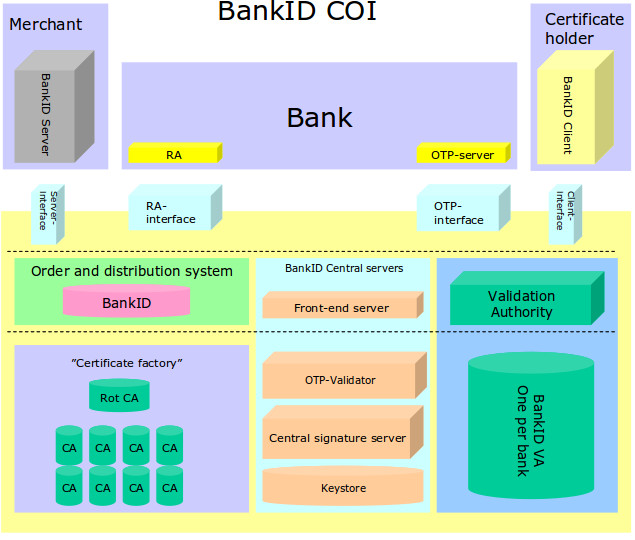
\includegraphics[scale=0.35]{architecture} %Note: no use of .jpg file ending
  \vspace{-0.2cm}
  \caption{BankID architecture.}
  \label{fig:arch}
\end{wrapfigure}
\subsection{Components and Architecture of the BankID system.}
\paragraph{PKI, public key infrastructure} is often the preferred model for efficient and secure online services. Often accompanied by the use of several factors of authentication. The background for this approach is the guidance entitled \emph{Authentication in an Internet Banking Environment} ~\cite{auth-banking}. PKI is a widely used technique used to provide public encryption and verification(digital signatures). The normal way of implementing a PKI, is by supplying each entity with their own private key, whom only they have control of. And then distribute the corresponding public key used to verify signatures and encrypt data. The variation deployed by BankID, is that the private keys is stored in a central database in control of the banks. I will come back to how this simplification contradicts basic requirements of digital signatures in PKI. BankID simplifies the structure by storing the signing keys centrally as well as doing all the cryptographic function on the central server. In other words, no software or sensitive information is stored on the users computer. An overview of the architecture is displayed in \hyperref[fig:Alice]{figure~\ref*{fig:arch}}. We can divide the components shown into two main parts; the central infrastructure consists of storage databases for certificates, cryptographic keys, all the bank's CAs, the validating authority and interfaces towards both end-users and merchants. The cryptographic functions and validation of signatures is also carried out in this part. Then we have a distributed part, involving the BankID server which normally is part of a web service and the client running in the users browser. We also have the RA (registration authority), which is located at the banks internal system. This entity is used when a new user wants to obtain a certificate, thus registering with the central interface~\cite{bankid}.



\begin{wrapfigure}[16]{r}{0.50\textwidth}
  \centering
  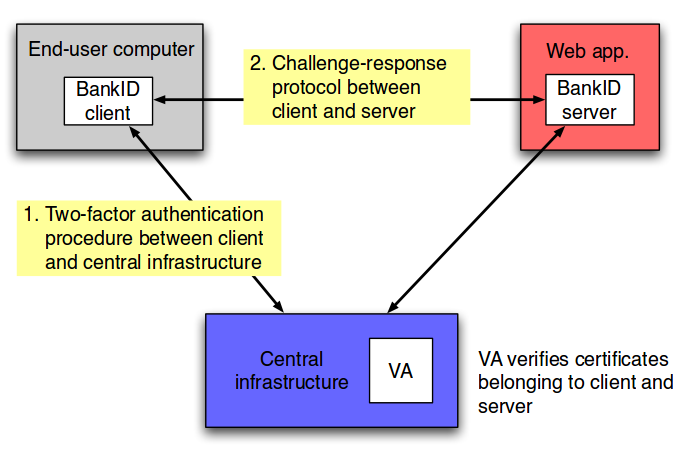
\includegraphics[scale=0.35]{flow} %Note: no use of .jpg file ending
  \vspace{-0.2cm}
  \caption{BankID authentication procedure.}
  \label{fig:flow}
\end{wrapfigure}
\paragraph{Two-factor authentication} is used to obtain mutual authentication between the bankID client and server. When performing authentication, the goal is to prove that you are who you claim to be. This is done using one or more \emph{factors} of authentication. The three basic factors used in authentication: \cite{auth-banking}:
\begin{itemize}
  \item A secret the user \emph{knows}, typically a user generated password/PIN. 
  \item Some device or secret the user \emph{has}, examples are the smart card piece of a normal visa card, or in the BankID case, the password generating token. 
  \item Something the user in himself \emph{is}, such as fingerprint or knowledge of some relationship between items.
\end{itemize}
The whole authentication procedure between client server and the third party is shown in \hyperref[fig:flow]{figure~\ref*{fig:flow}}. First the user enters his social security number which is used to generate a list of the users associated BankIDs (it is possible to have several). Then the client prompts the user for a one time password (OTP), generated by a password-generating token issued by the bank. This OTP is then verified at the central infrastructure, assuring the authenticity of the user. Next a static password is entered, which is used as a passphrase to gain access to the cryptographic keys~\cite{auth-banking}. Now the private keys can be used to authenticate with the server. 

The procedure described is a classic two-factor authentication process, with the factors being the OTP and the static password. Using two or more factors mitigates the problem of password getting stolen. Usually the OTP device generates passwords, which either change over time, or has a counter used to synchronise with the validator. If this password in some way is stolen, it wont be usable for the attacker. Newer systems has now started to look at mechanisms enabling the use of mobile phones as password generating tokens. This is implemented in the phone, with all the factors needed to generate the OTP stored in the phone and on the server. Factors such as identification number (IMSI or IMEI), timestamps (hour, minute, day) or other pseudorandom metrics are used to generate is often used when generating OTPs \cite{bankidmobil}.




\subsection{Security Capabilities}
 The main idea of this architecture is to enable two parties without a trusted relationship to establish a secure communication channel. We see that the establishment of the channel is done through a third party which both communicating parties trust. In classical PKIs this third party is a certificate authority (CA), which issues a certificate associating a public key to the recipient. In BankID, the public-private key pair is generated by the central infrastructure on request from the banks, typically when a new user is registered with BankID by the bank. The private key is stored in a central database as mentioned, while the public key is stored at the CA related to the customer's bank (may also be in the central infrastructure). When a user wants to use the BankID client, a Java applet in the browser is downloaded. The user is advised to check the certificate of this page, to assure the authenticity of the web page, and avoid phishing attacks. The user then authenticates with the server, and gives the central infrastructure access to the stored keys. Next, the infrastructure executes the actions requested (signing a challenge typically). The BankID server, being online stores or similar merchants can then verify the signed challenge received from the client and vice versa~\cite{auth-banking2}~\cite{bankid}. The two parties have now established a secure relationship, and the parameters sent, can't be used in replay attacks even if these were to be compromised. The central infrastructure can also be used to simply sign documents using the same functions. [TODO: strength of two-factor auth]  

\subsection{Vulnerabilities and Limitations.}
There are some limitations to the system regarding the central infrastructure. One fundamental requirement when using so called trust based PKI systems, is that the user should be in control of their own keypair \cite{digsig}. In a worst case scenario, this would open for a insider attack, since the banks is in total control of the users keys and certificates. There are some publications displaying attacks on the BankID system, but the banks claim to have fixed all of them. These attacks include man in the middle attacks, where the attacker sits between the customer and the infrastructure or BankID server. This attack exploits the assumption by the banks that users always check the certificate of the java application, which most users does not do. After tricking the user to authenticate through the MITM-server, the attacker relays the traffic until the authentication is completed. If the attacker wants to transfer money from the user's account, he will need one more OTP This can be done by alerting him that the first one was wrong, and therefore trick him into entering one more \cite{attack1}. This attack is most likely not feasible any more, but problems with the use of forms and we applications is still relevant. \\    
To biggest problem BankID encounters today is weaknesses in the Java platform, which the BankID client is depending on. Security breaches hitting the Java platform have been a major problem for BankID lately, causing them to lose customers and reputation. 





\section{Conclusion}
When dealing with high risk transactions involving sensitive user data and especially movement of funds, demands security on the highest possible level. I think that a move towards a more user controlled system would benefit all parties involved. The usage of user installed software like Java, may not be a big problem in itself, but it is still a unnecessary dependency, which only makes for more possible vulnerabilities.
It seems that BankID agrees with these suggestions, as they are moving more towards the said solution, using "BankID on mobiles", which is a lunge towards a more user controlled system, where the private key and certificate is stored in control of the user \cite{bankidmobil2}. BankID also announced their BankID 2.0 \cite{bankid2} earlier this year, in which they plan to phase out java completely. \\




\begin{thebibliography}{N}\label{sec:references}

\bibitem{auth-banking} Federal Financial Institutions Examination Council  \textit{Authentication in an Internet Banking Environment} 13-Sep-2011 \url{http://www.digitallibrary.kcci.com.pk/handle/32417747/701}

\bibitem{whitepaper} Bankenes BetalingsSentral AS \textit{BankID COI White Paper} 05.09.2005 \url{http://www.eurim.org.uk/activities/pi/BankIDWhitePaper.pdf}

\bibitem{bankid}  Professor K. J. Hole, Department of Informatics, University of
Bergen \textit{Next Generation Internet Banking in Norway} \url{https://bora.uib.no/bitstream/handle/1956/2636/Dr.Avh._Thomas_%20Tjostheim.pdf?sequence=1#page=141}

\bibitem{auth-banking2} IEEE SECURITY \& PRIVACY \textit{Secure Internet Banking Authentication} The IEEE Computer Science, March/April 2006 \url{http://ieeexplore.ieee.org/stamp/stamp.jsp?tp=&arnumber=1621056}

\bibitem{2-factor-auth} B. Schneier, \textit{Two-Factor Authentication: Too Little, Too Late}. AprilRisks 02.18.2005. \url{http://www.itsec.gov.cn/webportal/download/2004_two-factor.pdf}

\bibitem{bankidmobil}  Fadi Aloul, Syed Zahidi, Wassim El-Hajj, \textit{Two factor authentication using mobile phones,} Computer Systems and Applications, IEEE/ACS International Conference on Computer Systems and Applications, 2009 \url{http://ieeexplore.ieee.org/stamp/stamp.jsp?tp=&arnumber=5069395}

\bibitem{digsig} Directive 1999/93/EC of the European Parliament and of the Council of 13 December 1999 on a Community framework for electronic signatures \textit{Official Journal L 013 , 19/01/2000} \emph{Article 2} \url{http://eur-lex.europa.eu/LexUriServ/LexUriServ.do?uri=CELEX:31999L0093:en:HTML}

\bibitem{attack1}NoWires Research Group, Department of Informatics UiB \textit{A Proof of Concept Attack against Norwegian Internet Banking Systems} Short paper version, Feb. 21st, 2008.

\bibitem{bankidmobil2} BankID Norge \textit{BankID på mobil} (In Norwegian.) \url{https://www.bankid.no/Dette-er-BankID/BankID-pa-mobil/} Read 19.11.13

\bibitem{bankid2} BankID Norge \textit{BankID 2.0 blir Java-fri} (In Norwegian) \url{https://www.bankid.no/Presse-og-nyheter/Nyhetsarkiv/2013/BankID-20-blir-Java-fri/} Published: 26.04.2013, 08:40



\end{thebibliography}

\end{document} 
